% =============================================================================
% 2.2 基于 ReAct 范式的单智能体思维链模型解决方案
% 草稿版本：v0.3 (2026-05-07)
%   v0.1：完成正文初稿。\reffig{fig:agent-architecture} 以 \fbox 占位框给出。
%   v0.2：接入 figures/agent_architecture.png 真实出图，移除 \fbox 占位。
%   v0.3：按导师意见 10 在 2.2.1 末段嵌入 fig:react-loop ReAct 循环图，
%        承接思考-行动-观察循环的论述并衔接 2.2.3 总体架构。
% 字数：约 2000 字
% 风格规则：v0.2 风格（无 \textbf / \textit / 引例括号 / 双引号 / 破折号）
% 引用：\cite{ref13, ref15, ref18, ref19, ref30}
% 图表：
%   - 图 \reffig{fig:react-loop}             ReAct 推理-行动-观察循环图
%   - 图 \reffig{fig:agent-architecture}     气象 Agent 总体架构图
%   - 表 \reftab{tab:single-vs-multi-agent}  单智能体与多智能体的取舍对照
% 依赖宏包：booktabs / tabularx / graphicx（主稿已加载）
% =============================================================================

\subsection{基于 ReAct 范式的单智能体思维链模型解决方案}
\label{sec:react-paradigm}

\ref{sec:problem-modeling} 节提出的三个研究问题不能由任意单一方法
独立解决。意图解析需要语言理解能力，工具调度需要结构化输出能力,
数值与引用兜底需要外部组件协作能力。本节论证 ReAct 范式作为统一
方法论框架的合理性，并给出本文气象 Agent 在单智能体形态下的总体
架构。

\subsubsection*{2.2.1 \quad 思维链与 ReAct 推理 - 行动 - 观察循环}

思维链 \cite{ref13} 是把复杂任务分解为一系列中间推理步骤的提示
工程范式。其核心观察是大语言模型在隐式直接生成最终答案时常常出错,
但如果通过提示让模型显式写出中间推理步骤，则能在算术、常识推理
与符号操作任务上取得显著的准确率提升。Wei 等 \cite{ref13} 提出的
思维链提示方法奠定了大语言模型作为推理引擎的基本能力假设。但纯
思维链的局限是模型只能依赖训练时的内部知识，无法访问实时信息或
执行外部计算，因此对于气象任务这种强依赖最新数据与权威标准的场景
不能直接套用。

ReAct \cite{ref18} 把思维链与工具调用结合起来。模型在每一轮的输出
分为思考 (Thought) 与行动 (Action) 两部分，思考用于分析当前状态
并决定下一步行动，行动以结构化形式给出工具名与参数；外部环境执行
该行动并把结果作为观察 (Observation) 返回给模型，模型据此进行下一
轮思考。这种推理 - 行动 - 观察的交替循环把模型从纯生成者升级为
带工具的推理者，原本无法在内部完成的任务被拆解为多步外部协作。
本文气象 Agent 的核心循环采用 LangGraph 框架 \cite{ref15} 实现这一
范式，所有 11 个气象工具加 RAG 工具均通过同一个工具节点暴露给模型,
模型在每一轮自由选择是否调用、调用哪一个、传入什么参数。
ReAct 推理 - 行动 - 观察循环的整体形态见 \reffig{fig:react-loop}。

\begin{figure}[!ht]
    \centering
    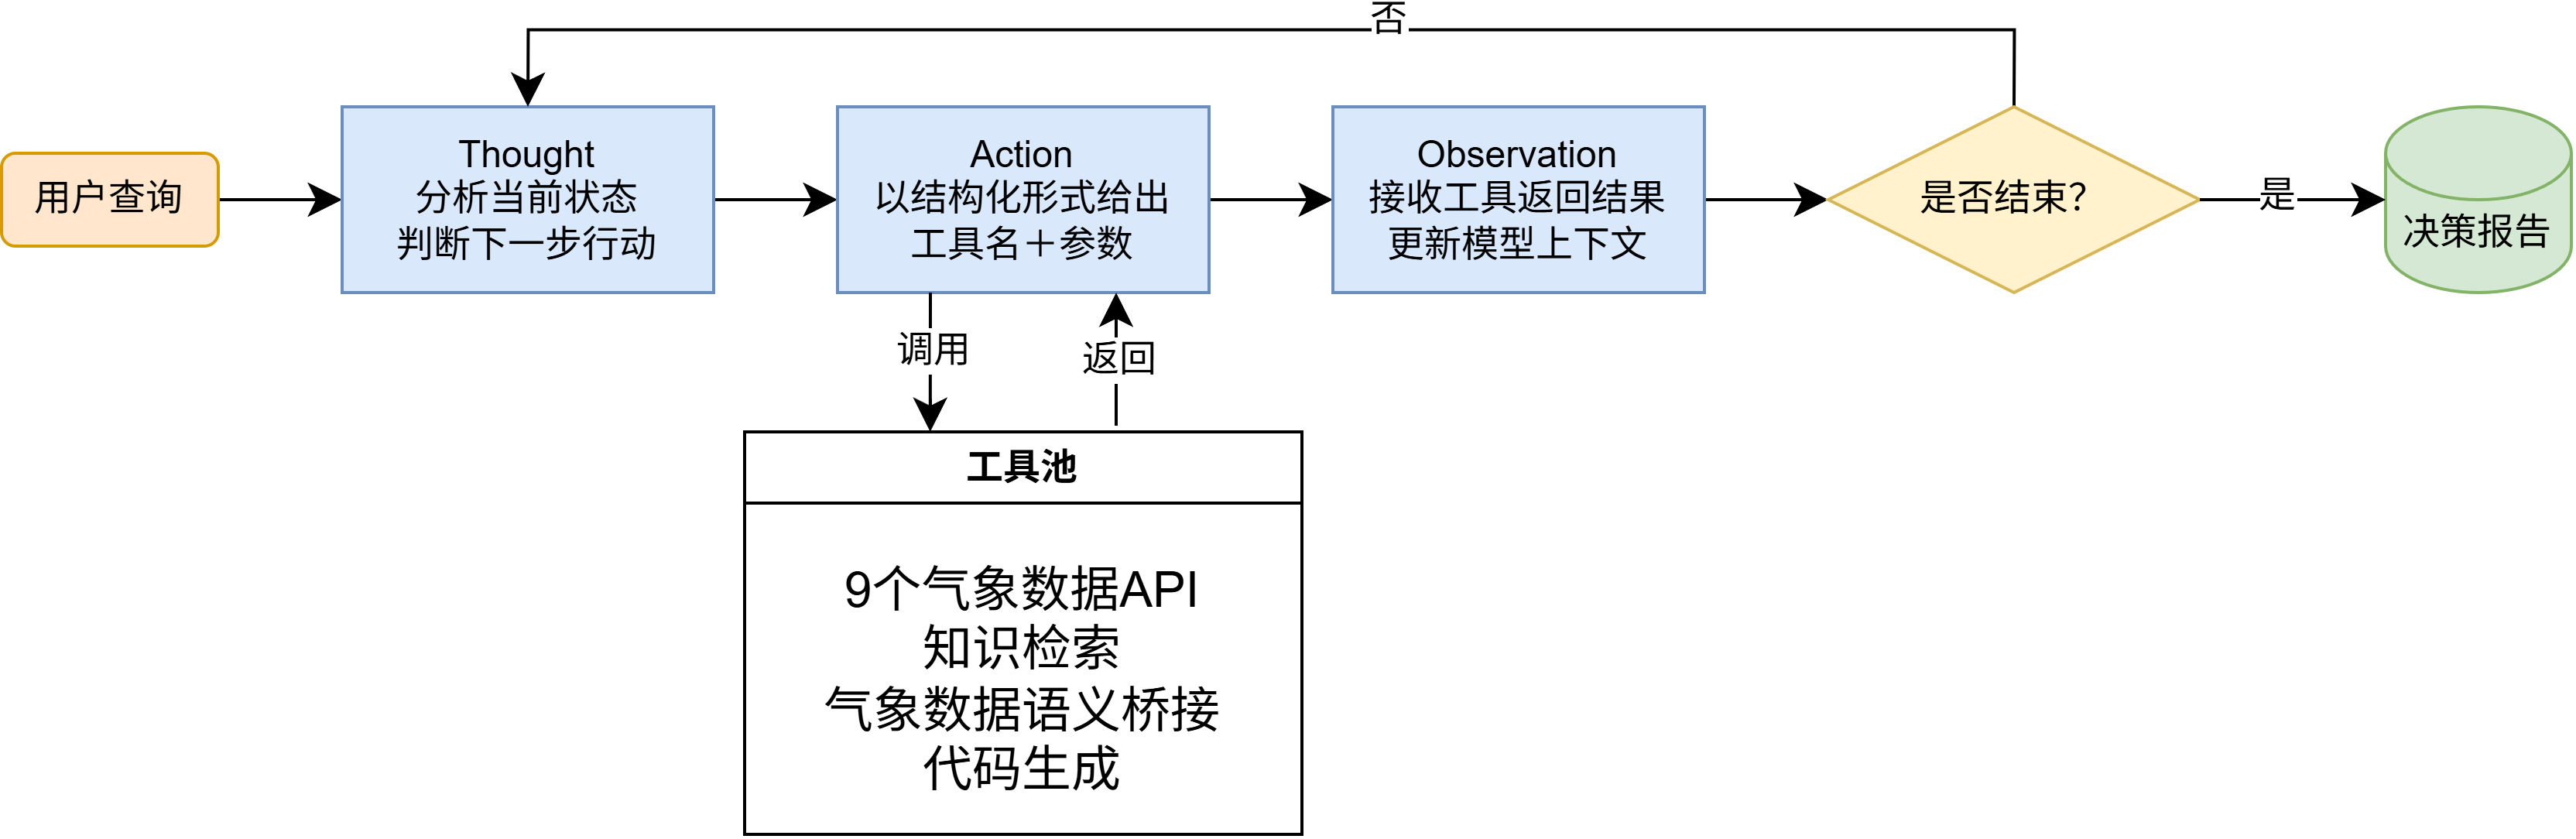
\includegraphics[width=0.85\linewidth]{figures/ReAct循环图}
    \caption{ReAct 推理-行动-观察循环示意图}
    \label{fig:react-loop}
\end{figure}

针对气象 Agent 的具体场景，本文在原始 ReAct 循环之上增加了三处
工程改造。第一是把意图识别与参数补全前置到 ReAct 循环之外作为
独立的 NLU 阶段，让 ReAct 循环以结构化 \texttt{WeatherIntent}
作为输入而非裸用户问题。这一改造对应指令解析问题，避免模型在
ReAct 循环内部承担意图与参数推理的双重负担。第二是把语义桥接
\texttt{bridge\_\bk{}weather\_\bk{}data} 工具与代码生成执行流水线作为
ReAct 循环可调用的子组件，让模型可以在拿到原始数值后主动选择是否
桥接、是否生成统计代码。这一改造对应数值与逻辑幻觉问题。第三是
显式记忆与状态保持。LangGraph 的 \texttt{InMemorySaver} 加
\texttt{thread\_\bk{}id} 机制让多轮对话中模型能继承上一轮的工具调用
结果与意图状态，避免每轮重复 search\_city 等基础查询。

Tree of Thoughts \cite{ref30} 在 ReAct 之外提出了搜索树形态的多
分支推理范式，更适合数学证明与谜题求解类任务。气象 Agent 的工具
调用任务在搜索深度与分支度上都不算大，单链 ReAct 循环已能覆盖
绝大多数场景，本文据此选择 ReAct 而非 Tree of Thoughts 作为基础
推理范式。

\subsubsection*{2.2.2 \quad 单智能体与多智能体的工程取舍}

近年来的 Agent 系统出现了从单智能体向多智能体协作演进的趋势。
AutoGen \cite{ref19} 提出可定制对话格局的多智能体框架，让多个具有
不同角色的 Agent 通过结构化对话协作完成复杂任务。本文不采用多
智能体方案，主要基于以下三点工程取舍，详见
\reftab{tab:single-vs-multi-agent}。

\begin{table}[!ht]
    \centering
    \caption{气象 Agent 单智能体与多智能体的工程取舍对照}
    \label{tab:single-vs-multi-agent}
    \song\fontsize{9pt}{12pt}\selectfont
    \renewcommand{\arraystretch}{0.95}
    \begin{tabular}{lll}
        \toprule
        维度 & 单智能体 & 多智能体 \\
        \midrule
        响应延迟 & 单进程内部循环 & 多 agent 间消息往返 \\
        状态同步 & 单一 \texttt{thread\_\bk{}id} 自动维护 & 需要显式协议 \\
        调试粒度 & 单条工具调用栈 & 跨 agent 日志关联 \\
        架构复杂度 & ReAct 单循环 & 角色定义加调度策略 \\
        适合任务 & 工具调用为主的查询 & 子任务分工明显的科研工作流 \\
        \bottomrule
    \end{tabular}
\end{table}

第一是响应延迟。气象 Agent 的典型查询从用户提问到最终回答需要在 5 至
15 秒内完成多步工具调用，目标用户对实时性的容忍度较低。多智能体
之间的消息传递引入额外的进程间或网络往返，对响应延迟敏感的查询
任务不友好。

第二是状态同步成本。气象 Agent 在多轮对话中需要保持地点状态、时间
状态、上次查询结果三类记忆。单智能体形态下这些状态由 LangGraph 的
\texttt{InMemorySaver} 在单一 \texttt{thread\_\bk{}id} 下自动累积，模型
不需要显式管理。多智能体形态下则必须额外定义状态同步协议，让规划
者、执行者、报告者三类角色看到一致的状态视图，工程开销显著上升。

第三是调试与可观测性。本文 5 套评测脚本统一以 ReAct 循环为入口,
单智能体形态下评测脚本可以直接复用 \texttt{run\_\bk{}agent} 函数,
故障定位时只需检查单一循环的中间状态。多智能体形态下故障可能发生
在任意子 Agent，需要跨 Agent 日志关联，调试成本与集成层不确定性
都会上升。

需要指出的是，本文的工具学习与语义桥接两个模块本身可以视为内嵌于
单智能体的子能力单元，承担了多智能体框架中规划者与执行者的部分
职责。这种把多智能体的角色专门化在单智能体内部以模块形式落地的
做法，在气象 Agent 这种工具调用为主的场景下既能保留模块化优势,
又规避了多智能体的延迟与同步开销。

\subsubsection*{2.2.3 \quad 气象 Agent 总体架构}

按上述方法论选型，本文气象 Agent 的总体架构由四个层次构成，整体
组件关系见 \reffig{fig:agent-architecture}。

\begin{figure}[!ht]
    \centering
    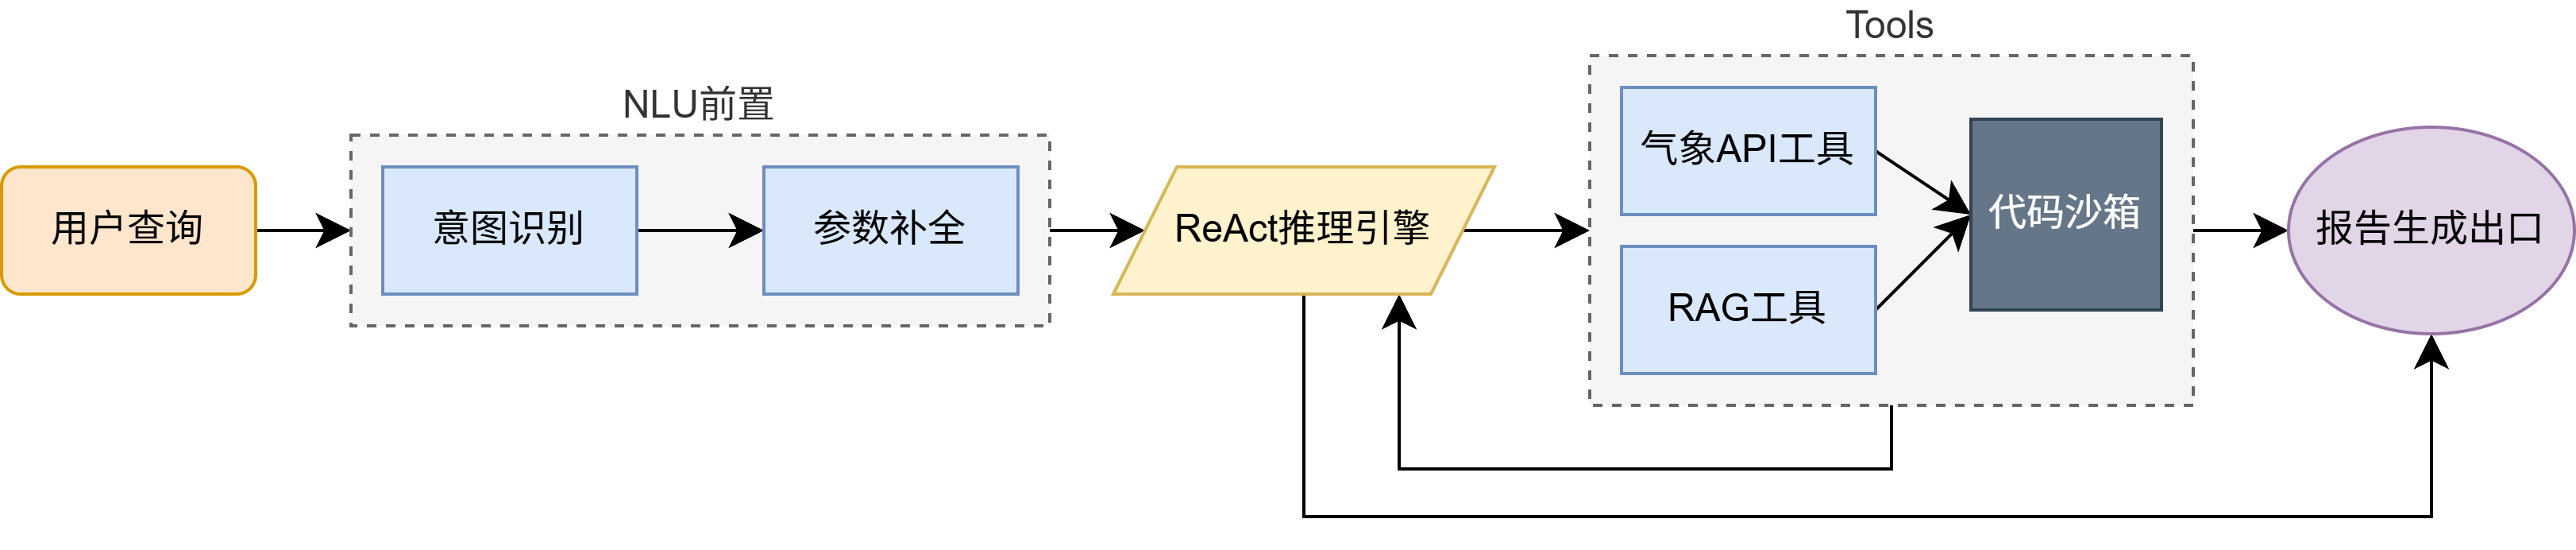
\includegraphics[width=\linewidth]{figures/agent_architecture}
    \caption{气象 Agent 总体架构示意图}
    \label{fig:agent-architecture}
\end{figure}

第一层是 NLU 前置层，由 \texttt{src/\bk{}intent/\bk{}recognizer.\bk{}py} 与
\texttt{src/\bk{}intent/\bk{}completer.\bk{}py} 两个模块构成，负责把用户自然语言
查询解析为 \texttt{WeatherIntent} 对象。这一层独立于 ReAct 循环
之外，让语言理解与工具执行解耦，便于独立评测与诊断（详见
\ref{chap:retrieval} 章）。

第二层是 ReAct 推理引擎，由 LangGraph \cite{ref15} 的
\texttt{create\_\bk{}agent} 实例化，以 SiliconFlow 提供的 GLM-5.1 为
底层大语言模型。推理引擎接收 NLU 前置层注入的结构化意图作为
首条用户消息，按 ReAct 范式 \cite{ref18} 在每一轮交替执行思考与
行动。System Prompt 以 117 行的长度承担工具调用规则、出行场景
推理规则、RAG 调用约束、输出规范四类硬约束，详见
\ref{sec:rag-prompt} 节。

第三层是工具与组件层，包含 11 个工具单元。9 个 \texttt{weather\_\bk{}api}
工具覆盖实时观测、逐小时与逐日预报、天气预警、生活指数、历史数据
六类业务场景；\texttt{search\_\bk{}knowledge} 工具从混合检索的 RAG
知识库中召回与查询相关的术语定义、分级标准、作业规范；
\texttt{bridge\_\bk{}weather\_\bk{}data} 工具把工具返回的原始数值经过确定性
分类器与 \texttt{grade\_\bk{}id} 硬链接转换为带引用源的语义标签。
此外，代码生成器与受限沙箱执行器作为第二级组件由前述工具按需
触发，承担确定性统计计算的兜底职责。

第四层是报告生成出口。Agent 在完成工具调用与中间推理后，由 LLM
按统一提示模板组织最终回答，要求显式引用知识库或桥接结果中的
权威条款，并在场景化模板下输出穿衣建议、出行建议、户外作业建议
或极端天气预警等结构化决策内容。

四个层次中，第一层与第三层的桥接、代码生成两个组件对应于本文的三
项核心创新（双阶段 NLU、双通路 RAG、代码生成与沙箱），第二层是
方法论框架，第四层是面向用户的最终出口。本文据此在第 3 章展开
第一层与第三层的工具学习子集，在第 4 章展开第三层的语义桥接、
代码生成与报告生成子集，在第 5 章对四个层次进行模块层与集成层
两个维度的系统化实证。

